% =====================================================================
%  Plant Disease Detection Menggunakan Lightweight Deep Learning
%  dengan Transfer Learning
%  Final Project Pembelajaran Mesin 2 — TI5 A2
%  Farrel Ghozy Affifudin (452024611053)
%  Universitas Darussalam Gontor
%  Format: IEEE Conference, A4, 2 kolom, maks 5 halaman
% =====================================================================
\documentclass[conference,a4paper]{IEEEtran}
\IEEEoverridecommandlockouts

\usepackage{cite}
\usepackage{amsmath,amssymb,amsfonts}
\usepackage{algorithmic}
\usepackage{graphicx}
\usepackage{textcomp}
\usepackage{xcolor}
\usepackage{booktabs}
\usepackage{multirow}
\usepackage{url}

\def\BibTeX{{\rm B\kern-.05em{\sc i\kern-.025em b}\kern-.08em
    T\kern-.1667em\lower.7ex\hbox{E}\kern-.125emX}}

\begin{document}

\title{Plant Disease Detection Menggunakan Lightweight Deep Learning dengan Transfer Learning: Studi Eksperimen pada Dataset PlantVillage}

\author{\IEEEauthorblockN{Farrel Ghozy Affifudin}
\IEEEauthorblockA{\textit{Teknik Informatika, Fakultas Sains dan Teknologi}\\
\textit{Universitas Darussalam Gontor}\\
Ponorogo, Indonesia \\
farrelghozyaffifudin@gmail.com}
}

\maketitle

\begin{abstract}
Penyakit tanaman merupakan salah satu faktor utama penurunan produktivitas pertanian, dan deteksi dini yang akurat menjadi kunci dalam pengendaliannya. Penelitian ini melakukan studi eksperimen klasifikasi 38 jenis penyakit dan kondisi sehat daun tanaman menggunakan arsitektur deep learning pada dataset PlantVillage (54.305 citra). Empat skenario eksperimen dibandingkan: (1) Custom CNN yang dilatih dari nol sebagai baseline, (2) MobileNetV3-Small dengan transfer learning dan backbone dibekukan, (3) EfficientNet-B0 dengan transfer learning dan backbone dibekukan, serta (4) MobileNetV3-Small dengan fine-tuning penuh. Seluruh model dilatih pada GPU NVIDIA RTX 4060 dengan konfigurasi training yang seragam (Adam, batch size 32, early stopping). Hasil menunjukkan bahwa MobileNetV3-Small dengan fine-tuning penuh mencapai akurasi test terbaik sebesar 98,99\% (F1 98,42\%), diikuti MobileNetV3-Small transfer learning dengan akurasi 97,47\%. Custom CNN baseline yang dilatih dari nol berada sedikit di atas EfficientNet-B0 yang backbone-nya dibekukan (95,09\% vs 94,98\%), mengindikasikan bahwa jumlah parameter trainable lebih menentukan daripada ukuran arsitektur pada dataset berskala besar. Analisis kesalahan menunjukkan confusi dominan antar kelas penyakit bercak daun (tomat dan jagung) yang memiliki kemiripan visual tinggi.
\end{abstract}

\begin{IEEEkeywords}
plant disease detection, deep learning, transfer learning, MobileNetV3, EfficientNet
\end{IEEEkeywords}

% =====================================================================
\section{Introduction}

Pertanian merupakan sektor strategis yang menyokong ketahanan pangan. Salah satu ancaman terbesar terhadap produktivitas pertanian adalah penyakit tanaman yang disebabkan oleh patogen seperti jamur, bakteri, dan virus. Keterlambatan dalam mendeteksi penyakit dapat menyebabkan penyebaran yang meluas dan kerugian hasil panen yang signifikan. Metode konvensional yang mengandalkan pengamatan visual oleh ahli patologi tanaman bersifat subjektif, memakan waktu, dan memerlukan keahlian khusus yang tidak selalu tersedia di daerah pedesaan.

Perkembangan deep learning, khususnya Convolutional Neural Network (CNN), telah membuka peluang besar dalam klasifikasi citra tanaman secara otomatis. Penelitian Mohanty dkk. [1] menunjukkan bahwa CNN mampu mengklasifikasikan penyakit tanaman dari citra daun dengan akurasi tinggi pada dataset PlantVillage. Namun demikian, model deep learning umumnya berukuran besar dan membutuhkan komputasi tinggi, sehingga kurang cocok untuk perangkat dengan sumber daya terbatas seperti smartphone.

Penelitian ini berfokus pada evaluasi arsitektur \emph{lightweight} yang cocok untuk perangkat edge, yaitu MobileNetV3-Small dan EfficientNet-B0, dengan memanfaatkan transfer learning. Kontribusi penelitian ini adalah: (1) perbandingan sistematis antara baseline CNN dari nol, transfer learning dengan backbone dibekukan, dan fine-tuning penuh pada dataset berskala besar; (2) analisis pengaruh jumlah parameter trainable terhadap performa; serta (3) error analysis untuk mengidentifikasi pola kesalahan klasifikasi antar kelas.

% =====================================================================
\section{Related Work}

Penelitian tentang deteksi penyakit tanaman berbasis deep learning telah banyak dilakukan. Mohanty dkk. [1] menggunakan arsitektur AlexNet dan GoogLeNet untuk mengklasifikasikan 26 penyakit pada 14 spesies tanaman dan mencapai akurasi hingga 99,35\% pada kondisi pengujian terkontrol. Ferentinos [2] mengevaluasi beberapa arsitektur CNN termasuk VGGNet dan ResNet pada dataset PlantVillage dan melaporkan akurasi di atas 99\%.

Untuk penerapan pada perangkat dengan sumber daya terbatas, arsitektur lightweight menjadi pilihan utama. Sandler dkk. [3] memperkenalkan MobileNetV2 dengan konsep \emph{inverted residual} dan \emph{linear bottleneck}, yang kemudian disempurnakan oleh Howard dkk. [4] melalui MobileNetV3 dengan \emph{Neural Architecture Search} (NAS). Tan dan Le [5] memperkenalkan EfficientNet dengan \emph{compound scaling} yang menyeimbangkan kedalaman, lebar, dan resolusi jaringan. Penelitian lain seperti Atila dkk. [6] menunjukkan bahwa EfficientNet mencapai akurasi tinggi pada klasifikasi penyakit tanaman, namun efektivitas pendekatan \emph{frozen backbone} versus \emph{fine-tuning} penuh pada dataset berskala besar masih perlu dieksplorasi lebih lanjut.

% =====================================================================
\section{Methodology}

\subsection{Dataset}
Penelitian ini menggunakan dataset PlantVillage [7] yang diperoleh dari Kaggle (Abdallah Ali, \emph{PlantVillage Dataset}, \url{https://www.kaggle.com/datasets/abdallahalidev/plantvillage-dataset}). Dataset terdiri dari 54.305 citra daun berwarna (RGB) yang terbagi dalam 38 kelas, mencakup 14 spesies tanaman (apel, tomat, kentang, anggur, jagung, dan lain-lain) dengan kondisi sehat dan berbagai penyakit. Distribusi citra antar kelas tidak seragam: kelas dengan jumlah citra terbanyak adalah Orange\_Haunglongbing (Citrus greening) (5.507 citra), sedangkan kelas terkecil adalah Potato\_healthy (152 citra), sehingga dataset bersifat \emph{imbalanced} pada tingkat tertentu.

Seluruh citra di-resize ke 224$\times$224 piksel. Pembagian data dilakukan secara \emph{stratified random split} dengan proporsi 80\% training (43.429 citra), 10\% validasi (5.417 citra), dan 10\% testing (5.459 citra).

\subsection{Preprocessing dan Augmentasi}
Citra dinormalisasi menggunakan mean dan standar deviasi ImageNet (mean = [0.485, 0.456, 0.406], std = [0.229, 0.224, 0.225]). Pada data training diterapkan augmentasi: \emph{random resized crop} (skala 0.8--1.0), \emph{horizontal flip}, rotasi acak $\pm 15^\circ$, dan \emph{color jitter} (brightness, contrast, saturation 0.2, hue 0.05). Data validasi dan testing hanya diberi resize 256 dan \emph{center crop} 224 tanpa augmentasi.

\subsection{Model Baseline: Custom CNN}
Baseline berupa CNN sederhana yang dilatih dari nol tanpa pretrained weights, terdiri dari empat blok konvolusi (32, 64, 128, 256 filter, masing-masing dengan batch normalization, ReLU, dan max-pooling 2$\times$2), dilanjutkan \emph{global average pooling}, dropout 0.5, fully-connected 512, dropout 0.3, dan output softmax 38 kelas. Total parameter 540.454, seluruhnya trainable.

\subsection{Model Transfer Learning}
Dua arsitektur lightweight pretrained ImageNet digunakan:
\begin{itemize}
\item \textbf{MobileNetV3-Small} [4]: total 1.556.806 parameter. Backbone dibekukan pada skenario E2 (hanya classifier yang dilatih, 629.798 parameter trainable) dan di-\emph{fine-tune} penuh pada skenario E4.
\item \textbf{EfficientNet-B0} [5]: total 4.056.226 parameter. Backbone dibekukan pada skenario E3 (hanya head yang dilatih, 48.678 parameter trainable).
\end{itemize}
Classifier diganti dengan fully-connected layer sesuai jumlah kelas (38).

\subsection{Konfigurasi Training}
Seluruh eksperimen menggunakan konfigurasi yang seragam: optimizer Adam, loss categorical cross-entropy, batch size 32, early stopping dengan patience 4 (monitor validation loss, \emph{restore best weights}), dan ReduceLROnPlateau (faktor 0.5, patience 2, minimum 1e-6). Training menggunakan mixed precision (FP16) pada GPU NVIDIA RTX 4060 (CUDA 12.4). Detail learning rate dan skenario eksperimen dijelaskan pada Bagian IV.

% =====================================================================
\section{Experimental Setup}

Empat skenario eksperimen dirancang untuk menjawab tiga pertanyaan: (1) seberapa baik baseline CNN dari nol pada dataset besar; (2) apakah transfer learning dengan backbone dibekukan lebih unggul; dan (3) apakah fine-tuning penuh memberikan peningkatan tambahan. Tabel \ref{tab:exp} merangkum desain eksperimen.

\begin{table}[htbp]
\caption{Desain Skenario Eksperimen}
\label{tab:exp}
\begin{center}
\begin{tabular}{@{}llll@{}}
\toprule
\textbf{Exp} & \textbf{Model} & \textbf{Strategi} & \textbf{LR} \\
\midrule
E1 & Custom CNN (0,54M) & Dari nol & $1\times10^{-3}$ \\
E2 & MobileNetV3-Small & TL, frozen & $1\times10^{-3}$ \\
E3 & EfficientNet-B0 & TL, frozen & $1\times10^{-3}$ \\
E4 & MobileNetV3-Small & TL, fine-tune & $1\times10^{-4}$ \\
\bottomrule
\end{tabular}
\end{center}
\end{table}

Metrik evaluasi yang digunakan adalah accuracy, precision, recall, dan F1-score (macro-averaged) pada test set, serta confusion matrix untuk analisis kesalahan per kelas. Epoch maksimum adalah 15 untuk E1 dan 12 untuk E2--E4, dengan early stopping sebagai penghenti dini.

% =====================================================================
\section{Results and Discussion}

\subsection{Perbandingan Performa Model}
Tabel \ref{tab:results} menampilkan hasil evaluasi keempat skenario pada test set (5.459 citra).

\begin{table}[htbp]
\caption{Hasil Evaluasi pada Test Set}
\label{tab:results}
\begin{center}
\begin{tabular}{@{}lcccc@{}}
\toprule
\textbf{Model} & \textbf{Acc} & \textbf{Prec} & \textbf{Rec} & \textbf{F1} \\
\midrule
E1: Custom CNN (baseline) & 0,9509 & 0,9485 & 0,9317 & 0,9339 \\
E2: MobileNetV3 frozen    & 0,9747 & 0,9679 & 0,9618 & 0,9641 \\
E3: EfficientNet-B0 frozen & 0,9498 & 0,9417 & 0,9319 & 0,9348 \\
\textbf{E4: MobileNetV3 fine-tune} & \textbf{0,9899} & \textbf{0,9881} & \textbf{0,9815} & \textbf{0,9842} \\
\bottomrule
\end{tabular}
\end{center}
\end{table}

Hasil menunjukkan bahwa seluruh model mencapai akurasi di atas 94\%, mengonfirmasi bahwa dataset PlantVillage relatif mudah dipelajari oleh CNN modern. MobileNetV3-Small dengan fine-tuning penuh (E4) menjadi model terbaik dengan akurasi test 98,99\% dan F1 98,42\%, diikuti MobileNetV3-Small dengan backbone dibekukan (E2) sebesar 97,47\%. Fine-tuning penuh memberikan peningkatan akurasi sebesar 1,52 poin persentase dibandingkan pendekatan frozen, karena seluruh representasi fitur ImageNet diadaptasi terhadap karakteristik citra daun. Kedua skenario MobileNetV3 mengungguli EfficientNet-B0 (E3) meskipun ukuran modelnya lebih kecil (1,56M vs 4,06M parameter).

Temuan yang menarik adalah Custom CNN yang dilatih dari nol (E1, 95,09\%) sedikit di atas EfficientNet-B0 dengan backbone dibekukan (E3, 94,98\%) meskipun arsitekturnya jauh lebih sederhana. Hal ini dapat dijelaskan oleh jumlah parameter trainable yang jauh berbeda: E1 melatih 540.454 parameter penuh, sedangkan E3 hanya melatih head 48.678 parameter. Dengan 43.429 citra training yang besar, model kecil yang dilatih penuh memiliki kapasitas yang cukup untuk mempelajari representasi spesifik dataset, sementara fitur ImageNet yang dibekukan pada EfficientNet-B0 tidak sepenuhnya optimal untuk karakteristik citra daun. Sebaliknya, MobileNetV3-Small (E2) memiliki classifier dua lapis (576$\rightarrow$1024$\rightarrow$38) dengan 629.798 parameter trainable yang lebih representatif, sehingga lebih unggul.

\subsection{Analisis Overfitting dan Underfitting}
Kurva training (Gambar \ref{fig:curves}) menunjukkan bahwa pada E4 (model terbaik) tidak terjadi overfitting yang signifikan: validation loss mencapai minimum 0,0244 di epoch 6, dan early stopping menghentikan training di epoch 10 setelah empat epoch tanpa perbaikan. Gap antara training dan validation accuracy tetap kecil (0,60 poin di epoch terakhir), dan training loss terus menurun hingga 0,0115 tanpa divergence. Pada E2 dan E3, selisih antara training dan validation accuracy juga relatif kecil dan validation loss menurun stabil. Pada E1, gap accuracy training-validation sedikit lebih besar namun tetap stabil, konsisten dengan kapasitas model yang lebih kecil. Penggunaan early stopping dan ReduceLROnPlateau mencegah overfitting pada epoch akhir seluruh skenario.

\begin{figure}[htbp]
\centering
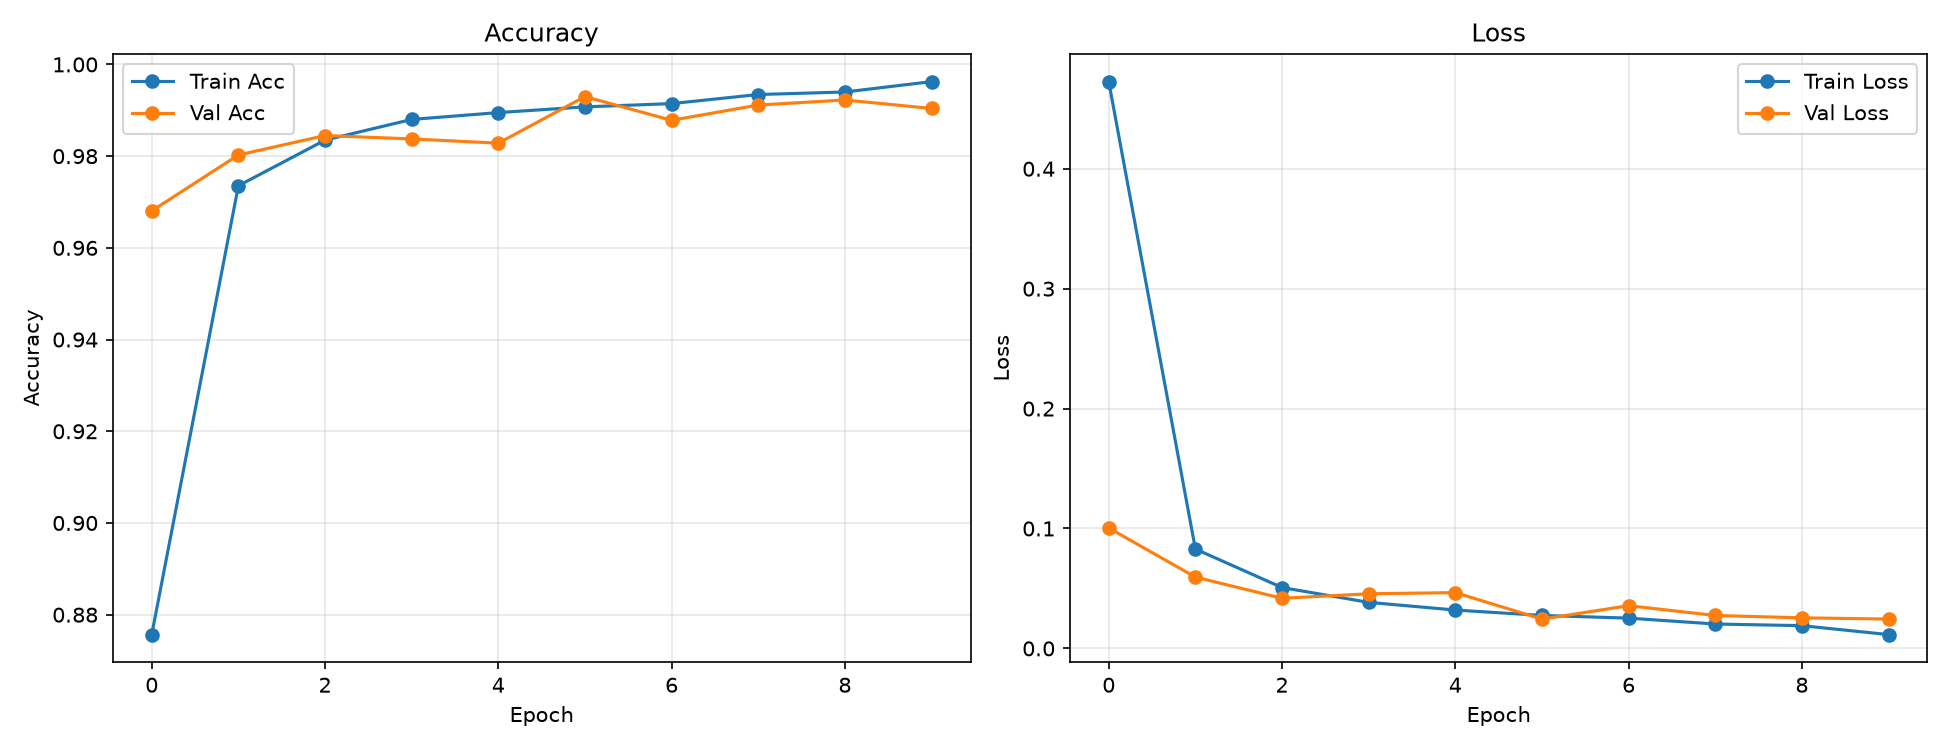
\includegraphics[width=\columnwidth]{../v2/results/e4/training_curves.png}
\caption{Kurva training dan validasi MobileNetV3-Small fine-tune (E4).}
\label{fig:curves}
\end{figure}

\subsection{Error Analysis}
Gambar \ref{fig:cm} menampilkan confusion matrix model E2 (transfer learning, backbone dibekukan). Model E2 dipilih untuk analisis kesalahan karena akurasinya yang tinggi (97,47\%) namun masih memiliki cukup banyak kesalahan untuk dianalisis polanya, berbeda dengan E4 yang confusion matrix-nya hampir diagonal sempurna. Analisis akurasi per kelas menunjukkan bahwa kelas terburuk adalah Potato\_healthy (75,00\%), diikuti Tomato\_Early\_blight (79,00\%), Corn\_Northern\_Leaf\_Blight (89,90\%), dan Tomato\_Spider\_mites (89,94\%). Pasangan kelas yang paling sering tertukar adalah:
\begin{itemize}
\item \emph{Tomato\_Early\_blight} $\rightarrow$ \emph{Tomato\_Septoria\_leaf\_spot}: kedua penyakit menimbulkan bercak nekrotik berwarna coklat pada daun tomat yang sulit dibedakan secara visual.
\item \emph{Corn\_Northern\_Leaf\_Blight} $\rightarrow$ \emph{Corn\_Cercospora\_leaf\_spot}: penyakit bercak daun jagung dengan pola lesi yang serupa.
\item \emph{Tomato\_Spider\_mites} $\leftrightarrow$ \emph{Tomato\_Target\_Spot}: kedua kelas saling tertukar, menunjukkan kemiripan pola bintik pada daun.
\item Confusi antar spesies: \emph{Tomato\_Bacterial\_spot} $\rightarrow$ \emph{Apple\_Apple\_scab} dan \emph{Orange\_Haunglongbing} $\rightarrow$ \emph{Soybean\_healthy}, mengindikasikan bahwa pada kasus tertentu model lebih mengandalkan tekstur daun daripada identitas spesies.
\end{itemize}

\begin{figure}[htbp]
\centering
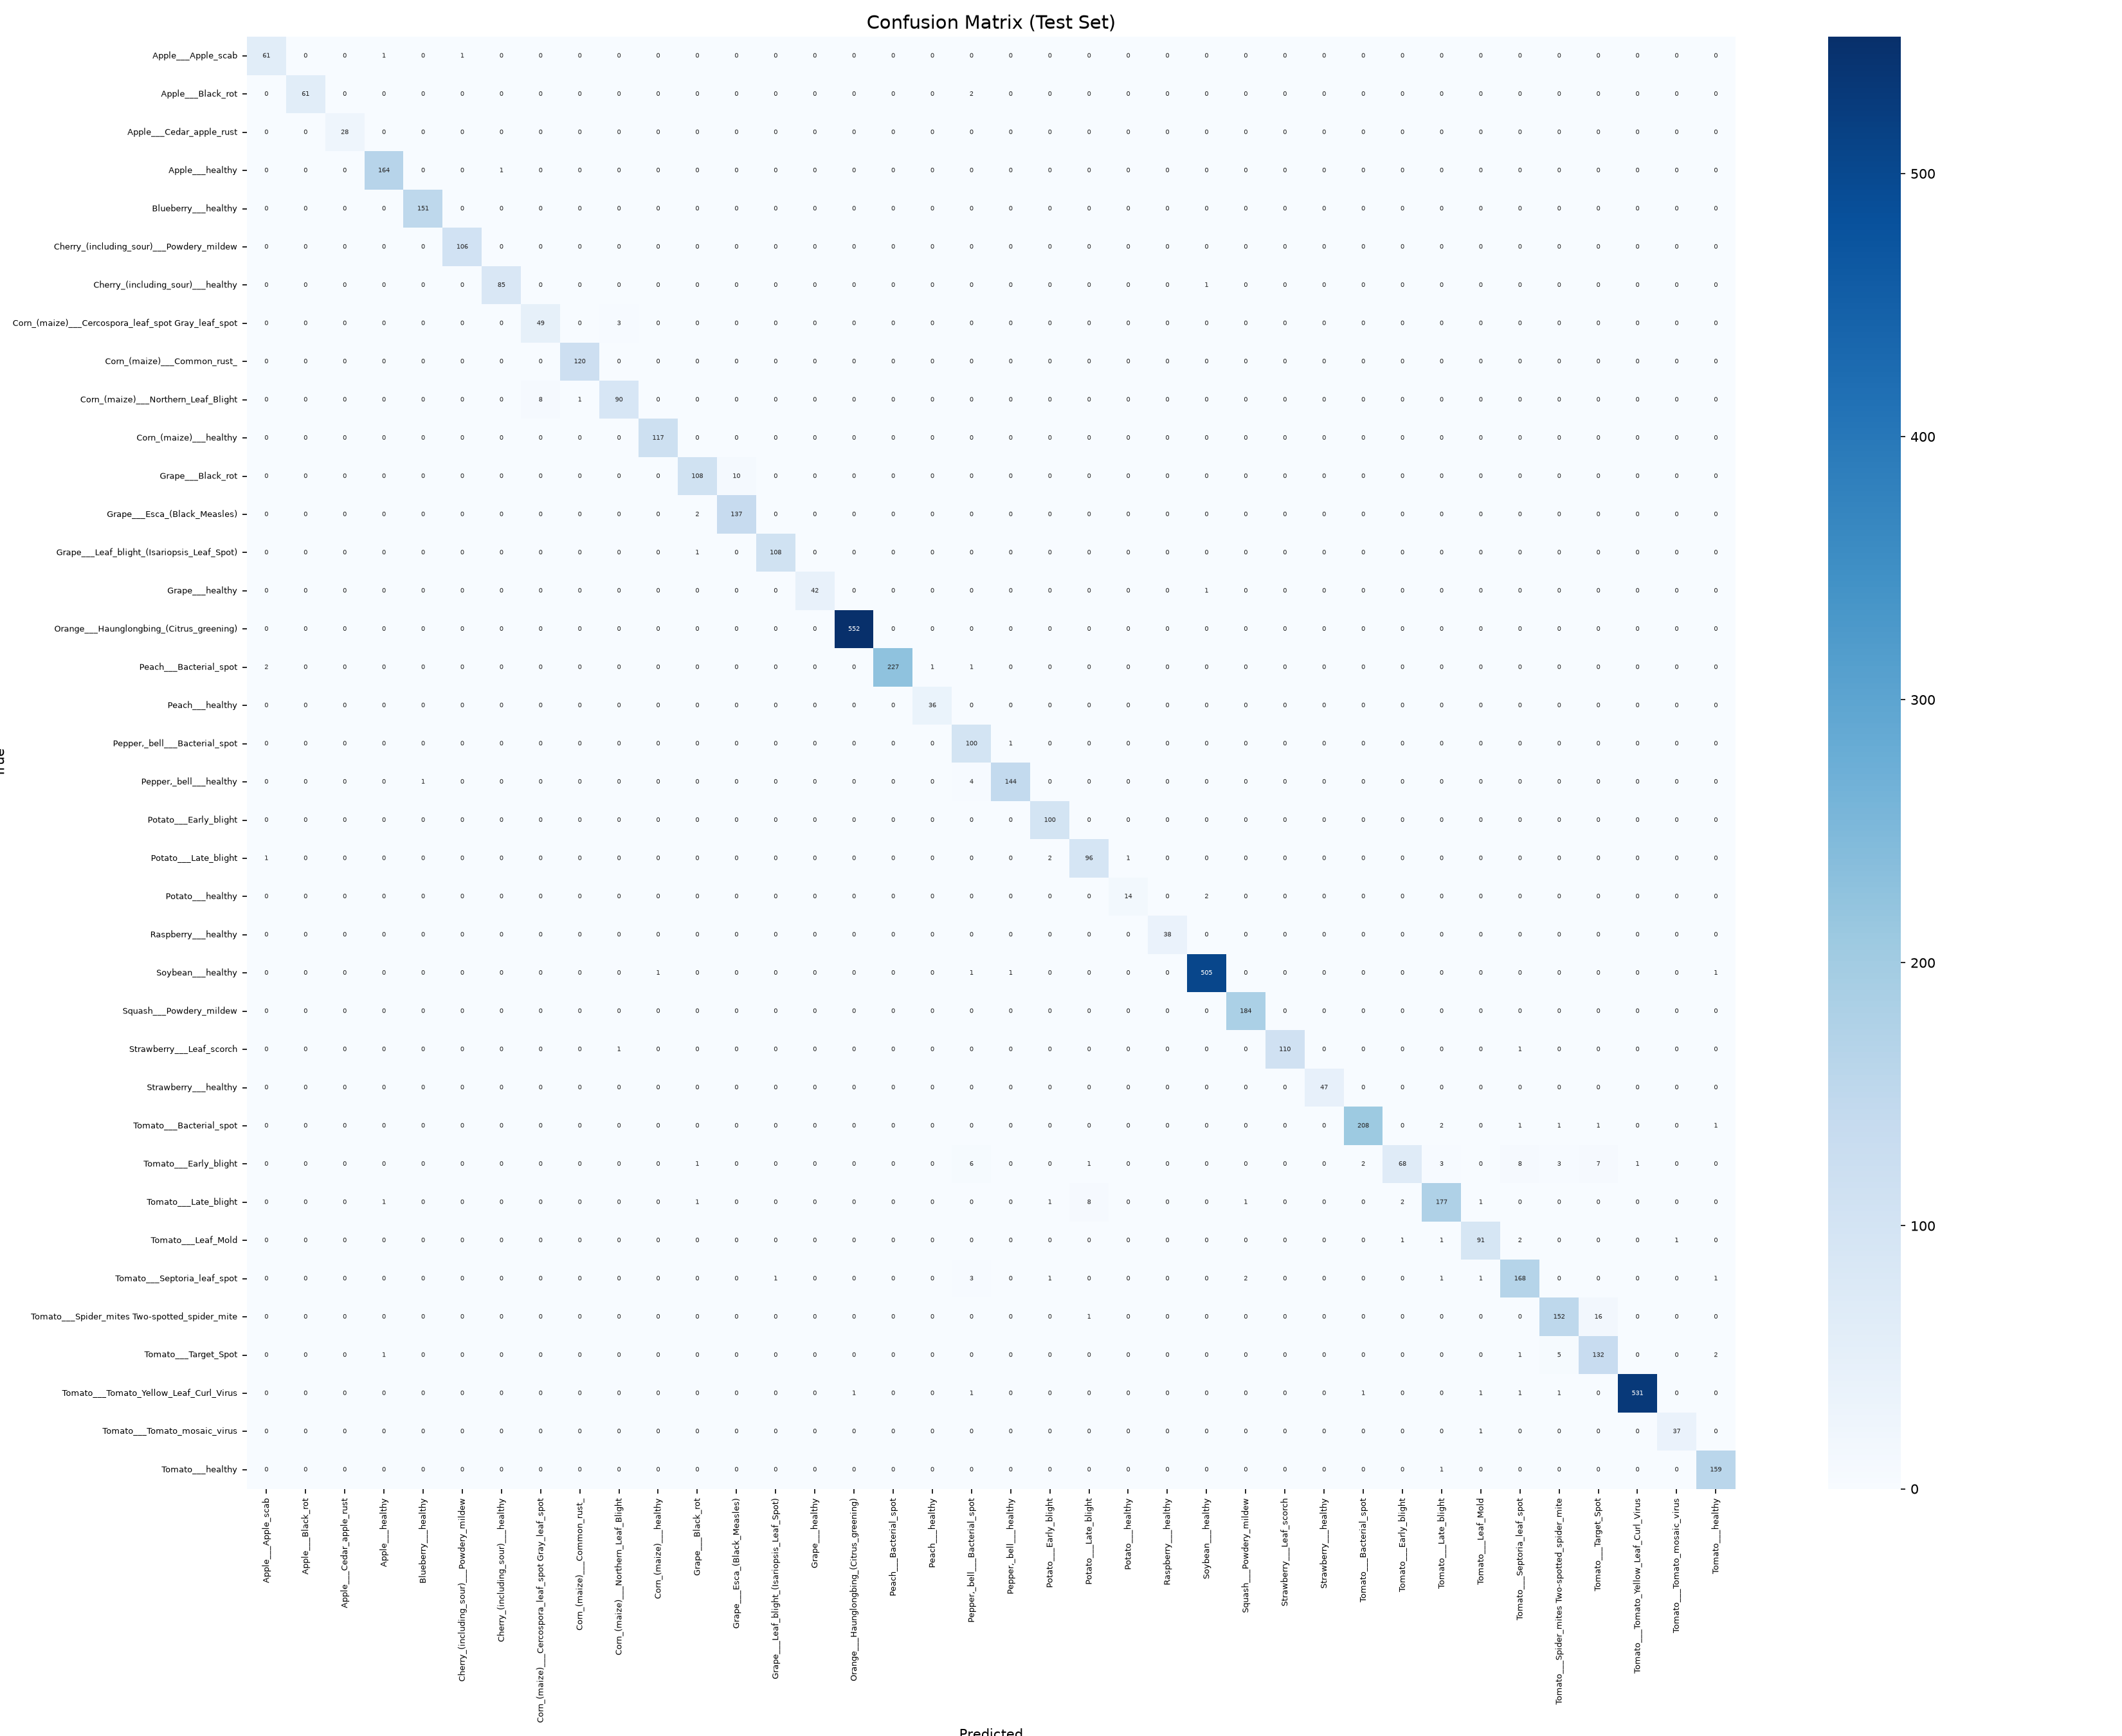
\includegraphics[width=\columnwidth]{../v2/results/e2/confusion_matrix.png}
\caption{Confusion matrix MobileNetV3-Small (E2) pada test set.}
\label{fig:cm}
\end{figure}

Confusi antar kelas sejenis tersebut wajar karena kelas-kelas tersebut berbagi latar belakang, tekstur, dan warna yang serupa. Keterbatasan utama model adalah ketergantungan pada latar belakang citra: citra PlantVillage sebagian besar diambil dengan latar seragam di laboratorium, sehingga performa pada citra lapangan yang lebih berisik belum teruji. Penelitian lanjutan dapat mengeksplorasi augmentasi domain acak, training pada citra lapangan, atau arsitektur dengan attention untuk membedakan kelas dengan kemiripan tinggi.

% =====================================================================
\section{Conclusion}

Penelitian ini mengevaluasi empat skenario eksperimen klasifikasi penyakit tanaman pada dataset PlantVillage (38 kelas, 54.305 citra) menggunakan arsitektur deep learning lightweight. MobileNetV3-Small dengan fine-tuning penuh mencapai akurasi test terbaik 98,99\% (F1 98,42\%), menjadikannya kandidat terbaik untuk penerapan pada perangkat edge. Eksperimen juga menunjukkan bahwa fine-tuning penuh meningkatkan akurasi sebesar 1,52 poin dibandingkan backbone yang dibekukan, dan jumlah parameter trainable lebih berpengaruh terhadap performa daripada ukuran arsitektur ketika dataset cukup besar: CNN baseline yang dilatih dari nol (95,09\%) sedikit di atas EfficientNet-B0 dengan backbone dibekukan (94,98\%). Keterbatasan penelitian ini adalah penggunaan dataset laboratorium yang relatif bersih; validasi pada citra lapangan dan eksplorasi augmentasi yang lebih agresif menjadi arah pengembangan selanjutnya. Untuk reproduksibilitas, seluruh source code, skrip eksperimen, dan hasil training (log, metrik, kurva, confusion matrix) tersedia pada \url{https://github.com/FarrelGhozy/TI5A2\_452024611053\_PembelanganMesin2\_FarrelGhozy}.

% =====================================================================
\section*{Acknowledgment}
Ucapan terima kasih disampaikan kepada dosen pengampu mata kuliah Pembelajaran Mesin 2 atas arahan dalam pelaksanaan penelitian ini.

\begin{thebibliography}{1}
\bibitem{mohanty2016}
S.~P. Mohanty, D.~P. Hughes, and M.~Salath{\'e}, ``Using deep learning for image-based plant disease detection,'' \emph{Frontiers in Plant Science}, vol.~7, p.~1419, 2016.

\bibitem{ferentinos2018}
K.~P. Ferentinos, ``Deep learning models for plant disease detection and diagnosis,'' \emph{Computers and Electronics in Agriculture}, vol.~145, pp.~311--318, 2018.

\bibitem{sandler2018}
M.~Sandler, A.~Howard, M.~Zhu, A.~Zhmoginov, and L.-C. Chen, ``MobileNetV2: Inverted residuals and linear bottlenecks,'' in \emph{Proc. IEEE/CVF Conf. Computer Vision and Pattern Recognition (CVPR)}, 2018, pp.~4510--4520.

\bibitem{howard2019}
A.~Howard, M.~Sandler, G.~Chu, L.-C. Chen, B.~Chen, M.~Tan, W.~Wang, Y.~Zhu, R.~Pang, V.~Vasudevan, Q.~V. Le, and H.~Adam, ``Searching for MobileNetV3,'' in \emph{Proc. IEEE/CVF Int. Conf. Computer Vision (ICCV)}, 2019, pp.~1314--1324.

\bibitem{tan2019}
M.~Tan and Q.~V. Le, ``EfficientNet: Rethinking model scaling for convolutional neural networks,'' in \emph{Proc. 36th Int. Conf. Machine Learning (ICML)}, 2019, pp.~6105--6114.

\bibitem{atila2021}
U.~Atila, M.~U{\c{c}}ar, K.~Akyol, and E.~U{\c{c}}ar, ``Plant leaf disease classification using EfficientNet deep learning model,'' \emph{Ecological Informatics}, vol.~61, p.~101182, 2021.

\bibitem{hughes2015}
D.~P. Hughes and M.~Salath{\'e}, ``An open access repository of images on plant health to enable the development of mobile disease diagnostics,'' \emph{arXiv preprint arXiv:1511.08060}, 2015.
\end{thebibliography}

\end{document}
